\subsection{Treeish}
\begin{frame}
    \frametitle{Treeish objects}
    \begin{figure}
        \begin{center}
            \ifnumequal{\aspectratio}{43}
            {
                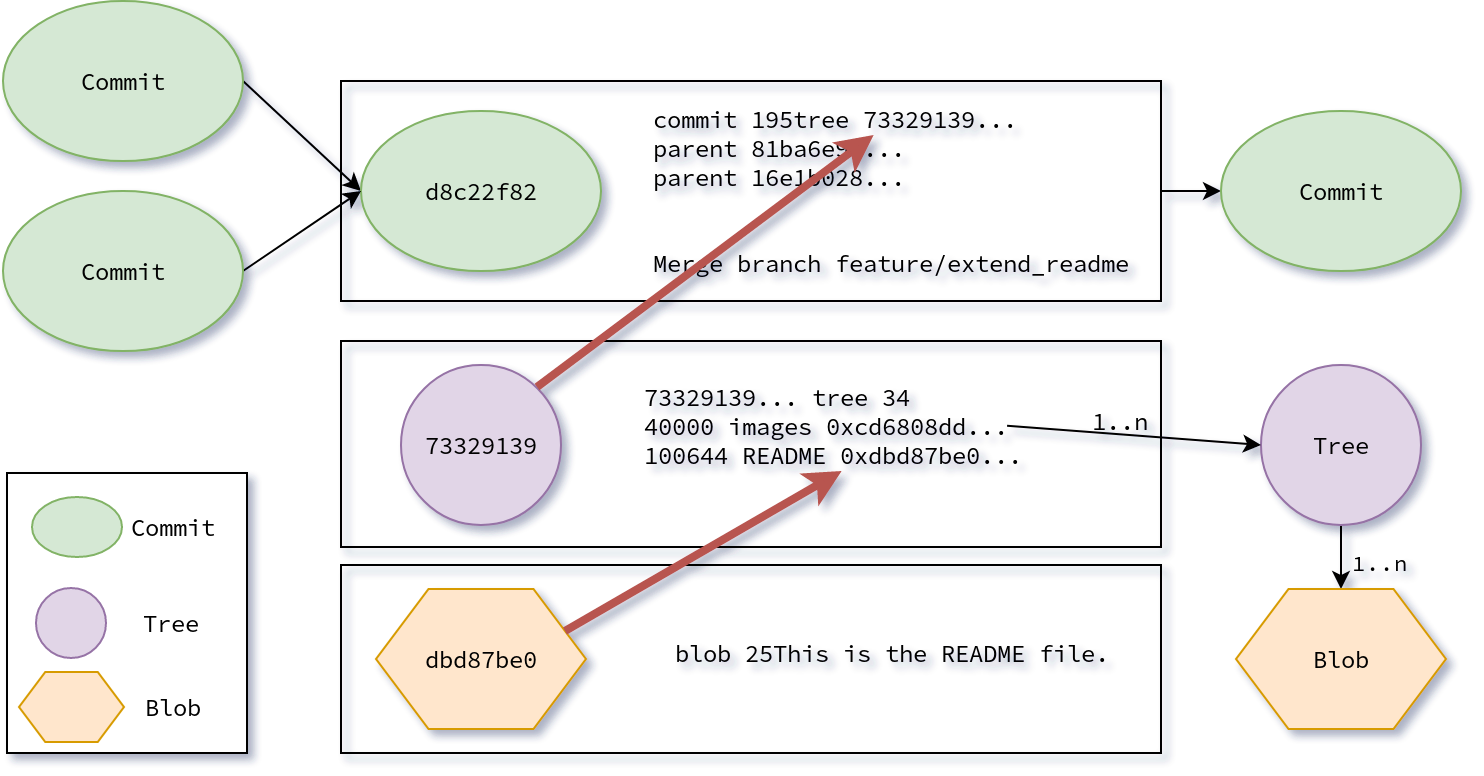
\includegraphics[height=0.70\textheight,keepaspectratio]{./images/Treeish.png}
            }
            {
                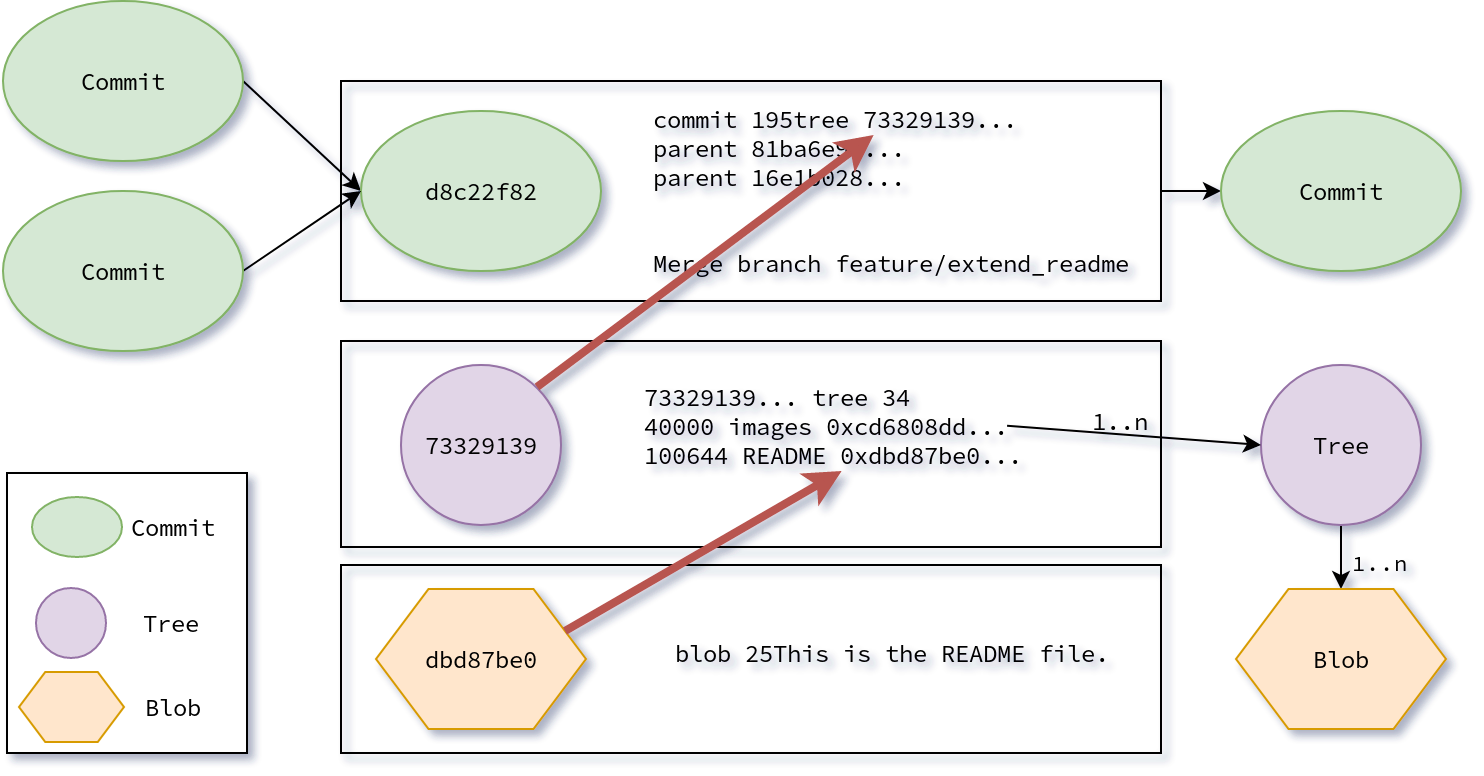
\includegraphics[height=0.6\textheight,width=0.8\textwidth]{./images/Treeish.png}
            }
            \caption{Git tree object explained}
        \end{center}
    \end{figure}
\end{frame}

\begin{frame}[noframenumbering]
    \frametitle{Treeish objects - commit}
    \addtocounter{page}{-1}
    \begin{figure}
        \begin{center}
            \ifnumequal{\aspectratio}{43}
            {
                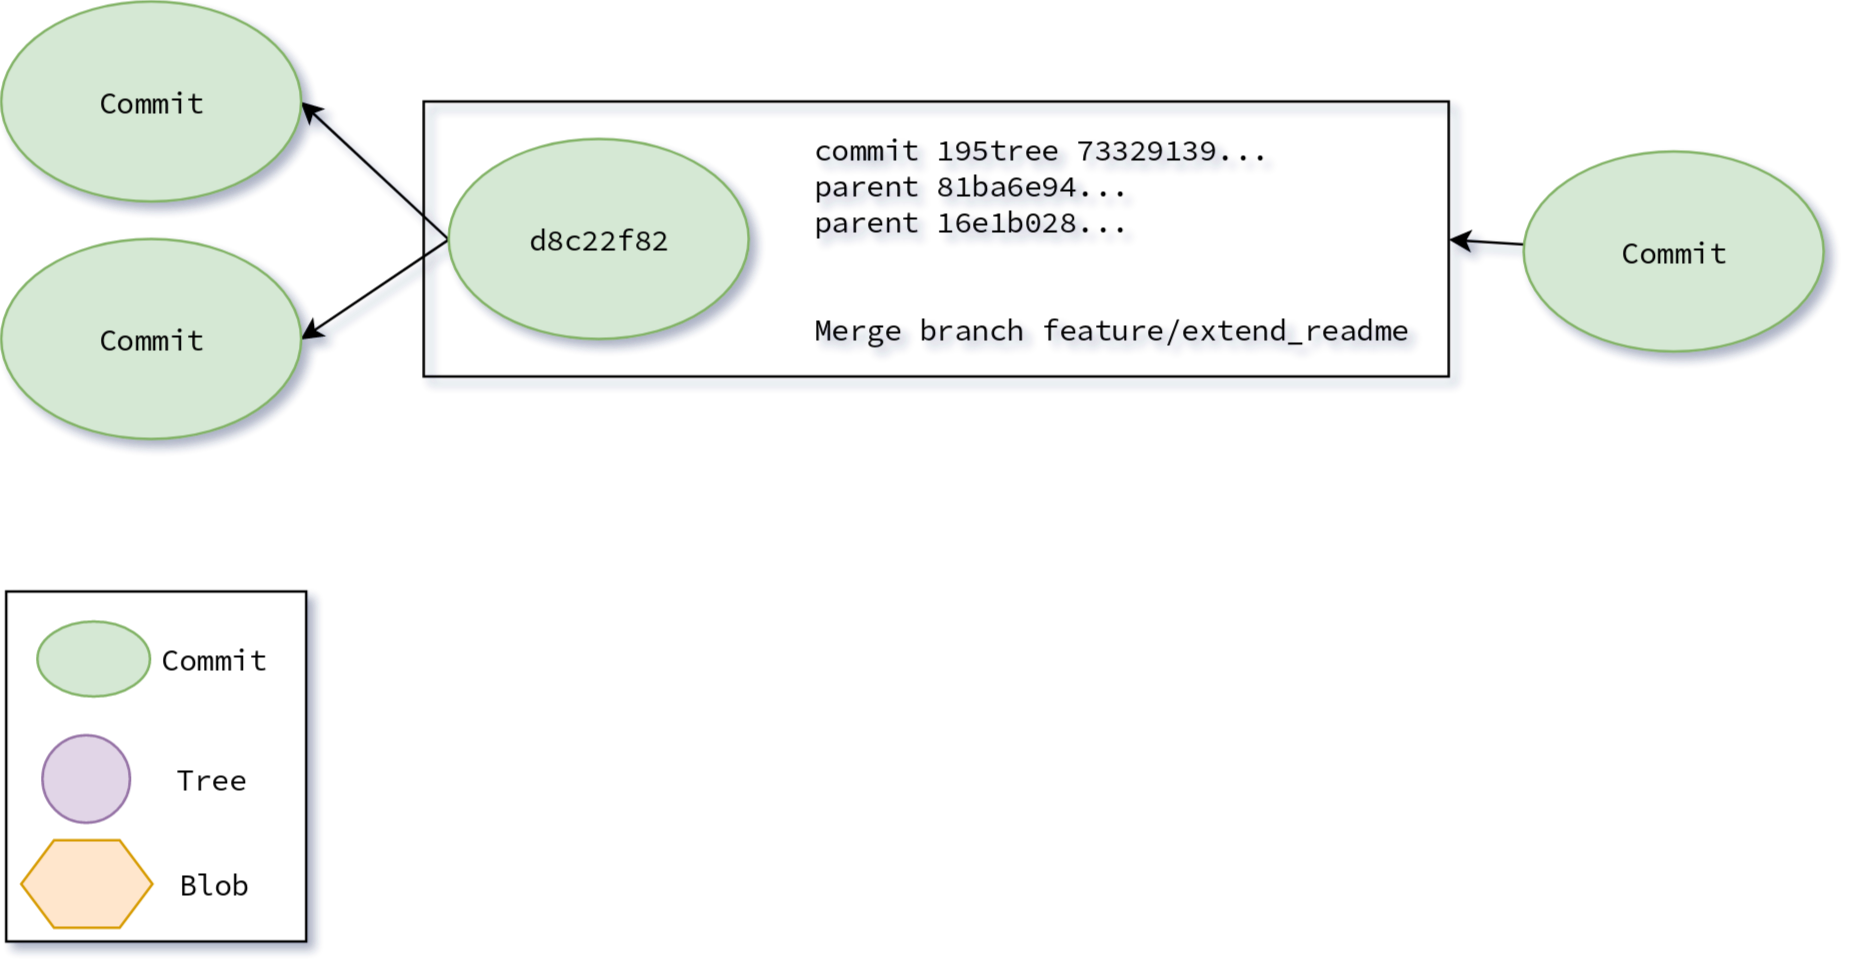
\includegraphics[height=0.70\textheight,keepaspectratio]{./images/Treeish_Commit.png}
            }
            {
                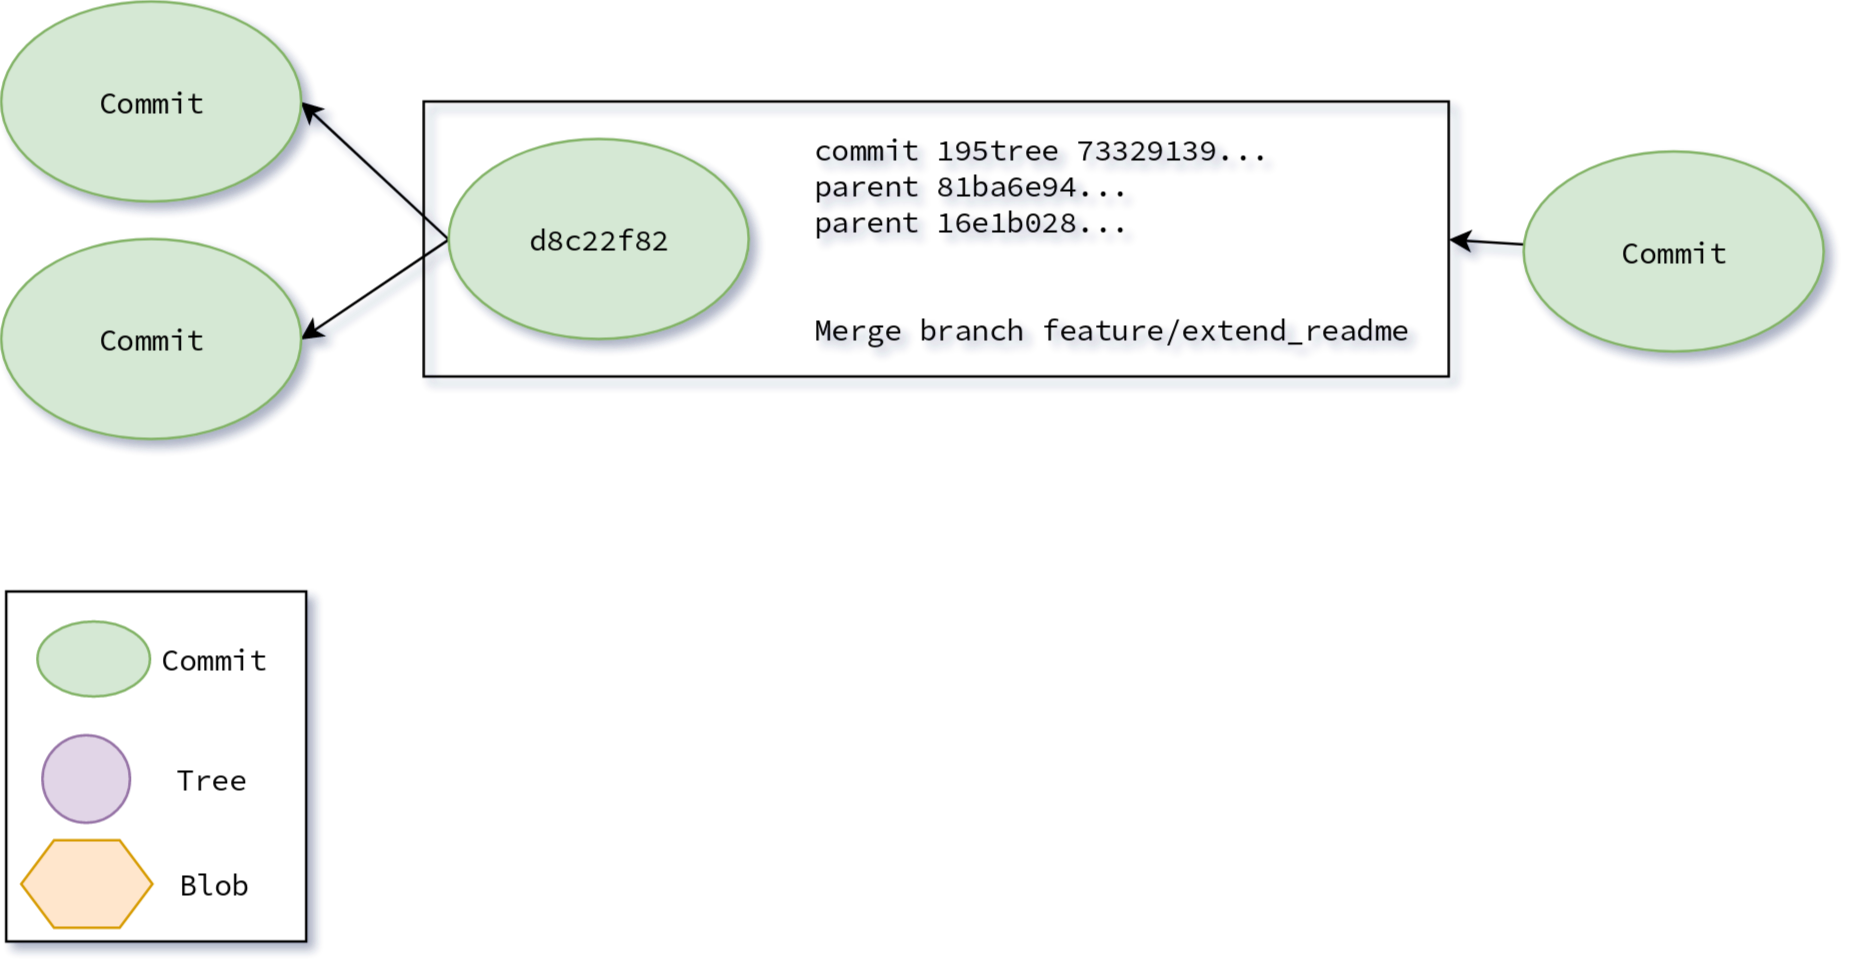
\includegraphics[height=0.6\textheight,width=0.8\textwidth]{./images/Treeish_Commit.png}
            }
            \caption{Git commit}
        \end{center}
    \end{figure}
\end{frame}

\begin{frame}[noframenumbering]
    \frametitle{Treeish objects - tree}
    \addtocounter{page}{-1}
    \begin{figure}
        \begin{center}
            \ifnumequal{\aspectratio}{43}
            {
                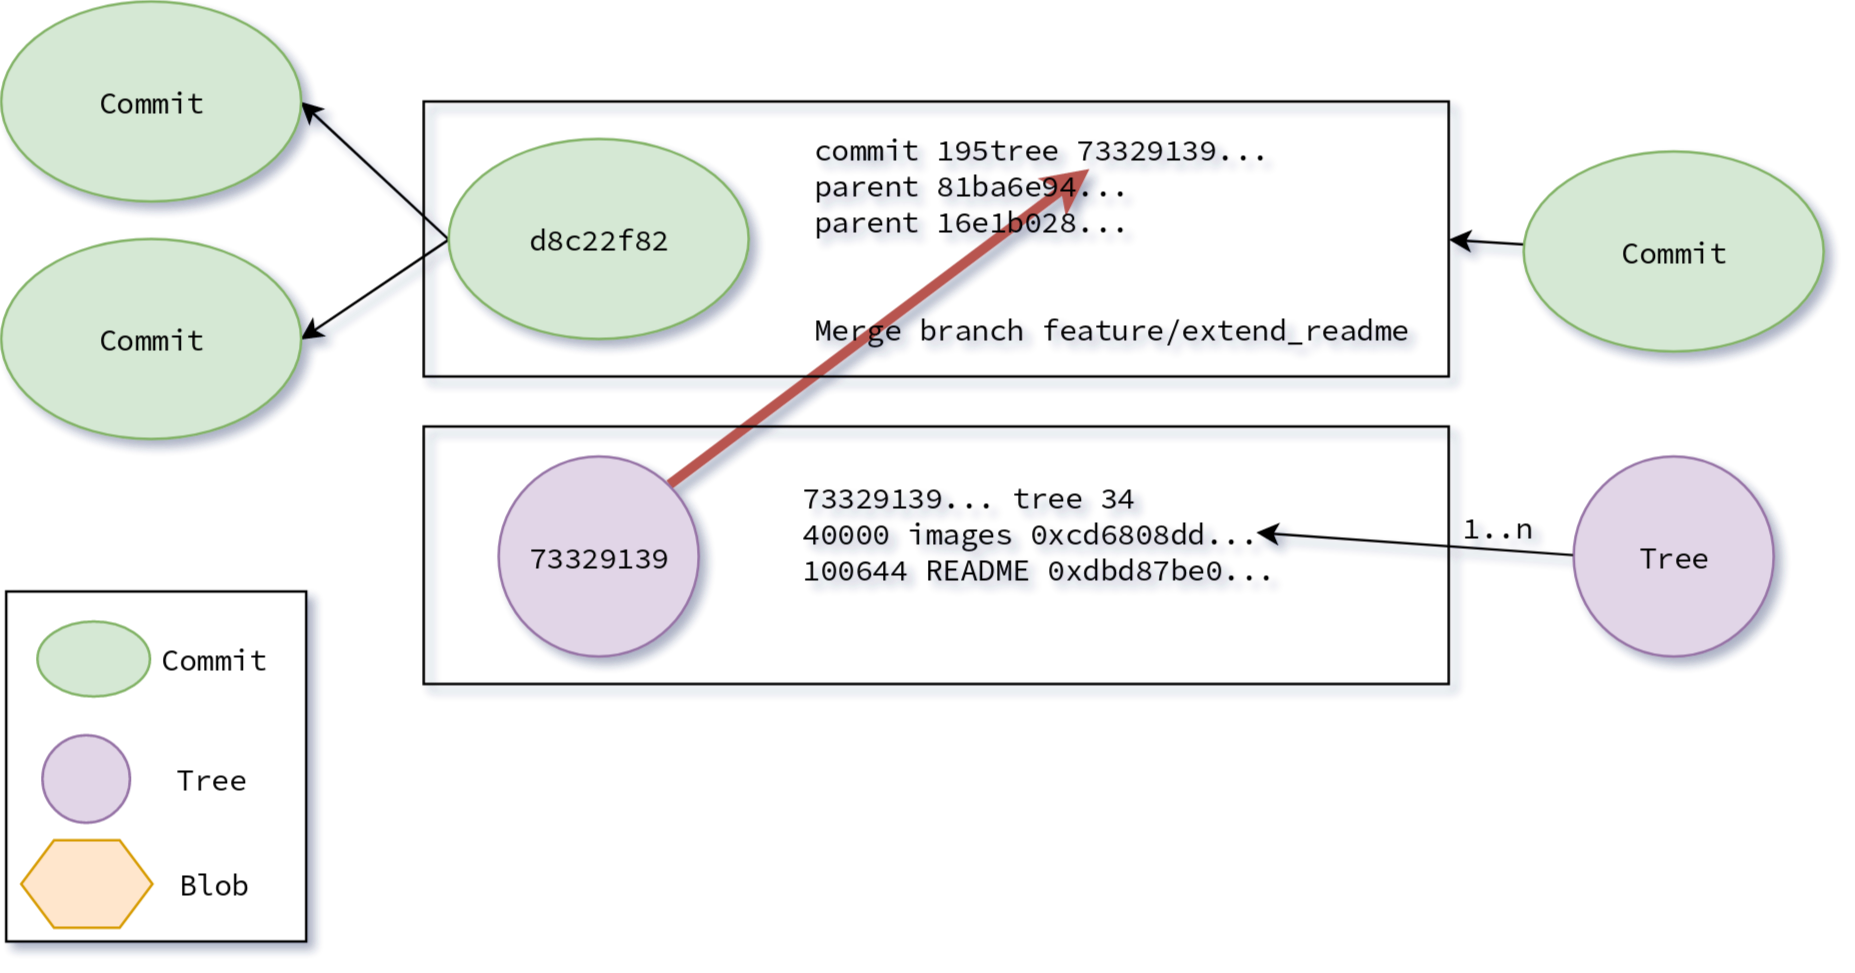
\includegraphics[height=0.70\textheight,keepaspectratio]{./images/Treeish_Tree.png}
            }
            {
                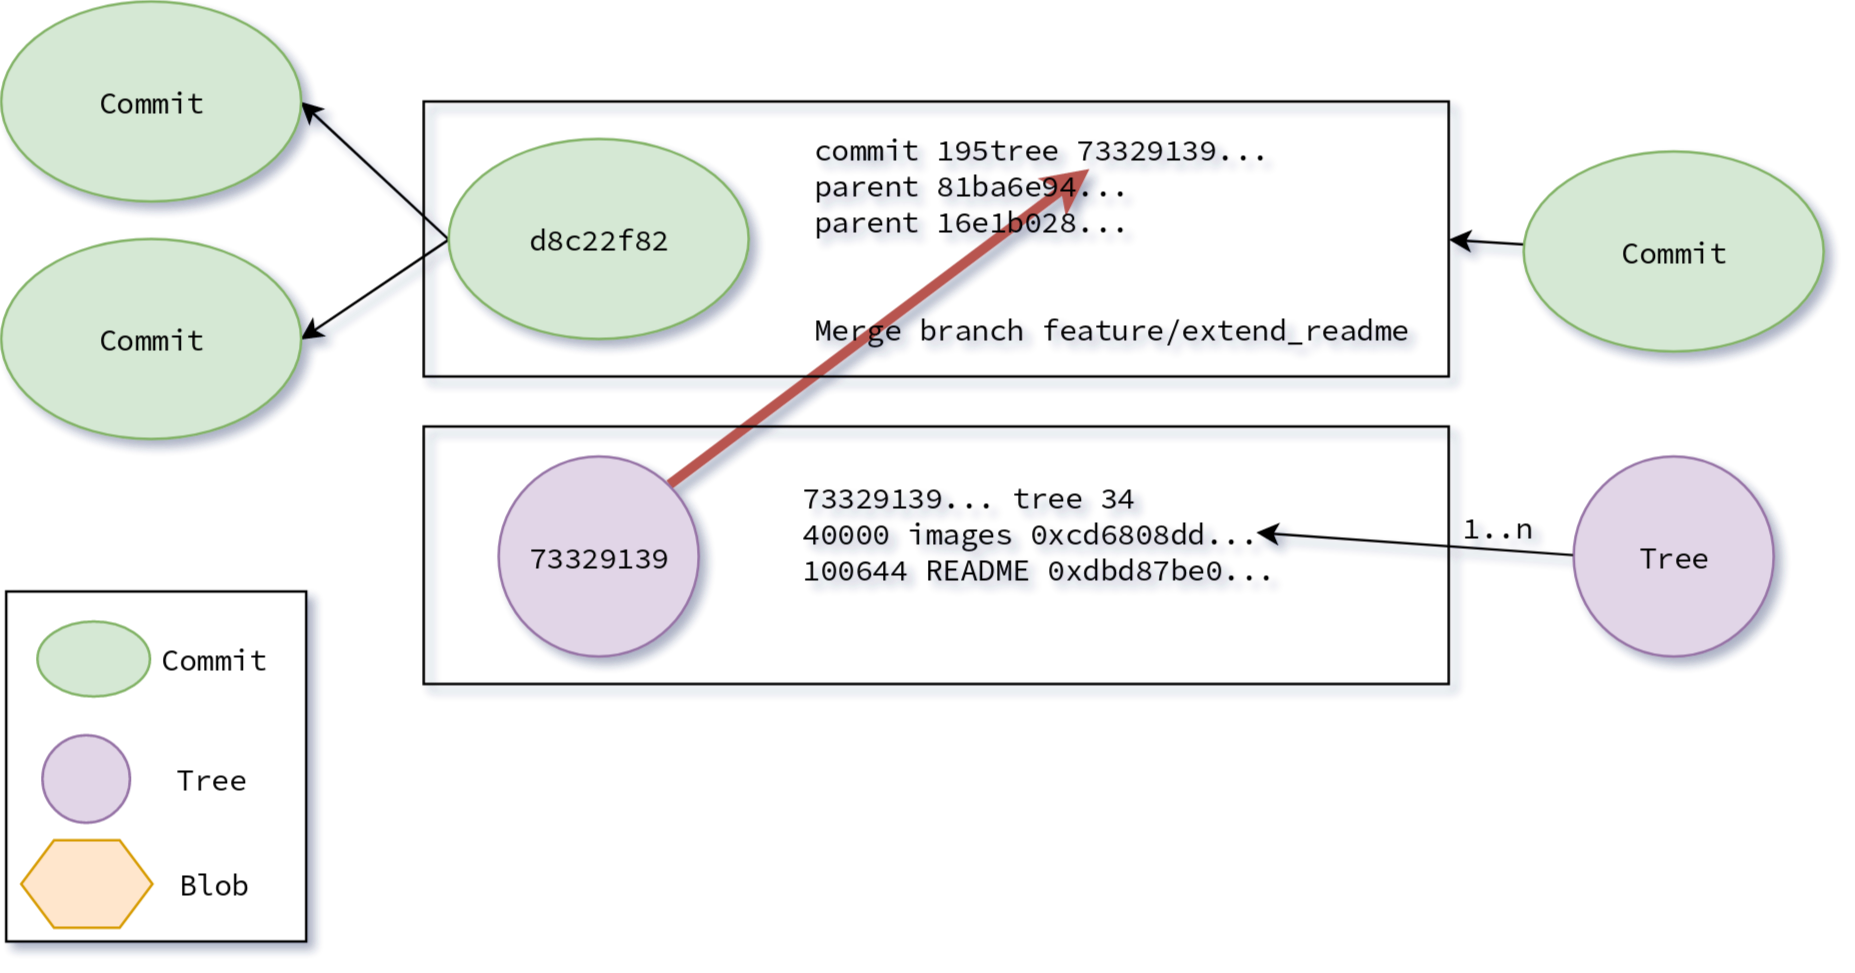
\includegraphics[height=0.6\textheight,width=0.8\textwidth]{./images/Treeish_Tree.png}
            }
            \caption{Git tree}
        \end{center}
    \end{figure}
\end{frame}

\begin{frame}[noframenumbering]
    \frametitle{Treeish objects - blob}
    \addtocounter{page}{-1}
    \begin{figure}
        \begin{center}
            \ifnumequal{\aspectratio}{43}
            {
                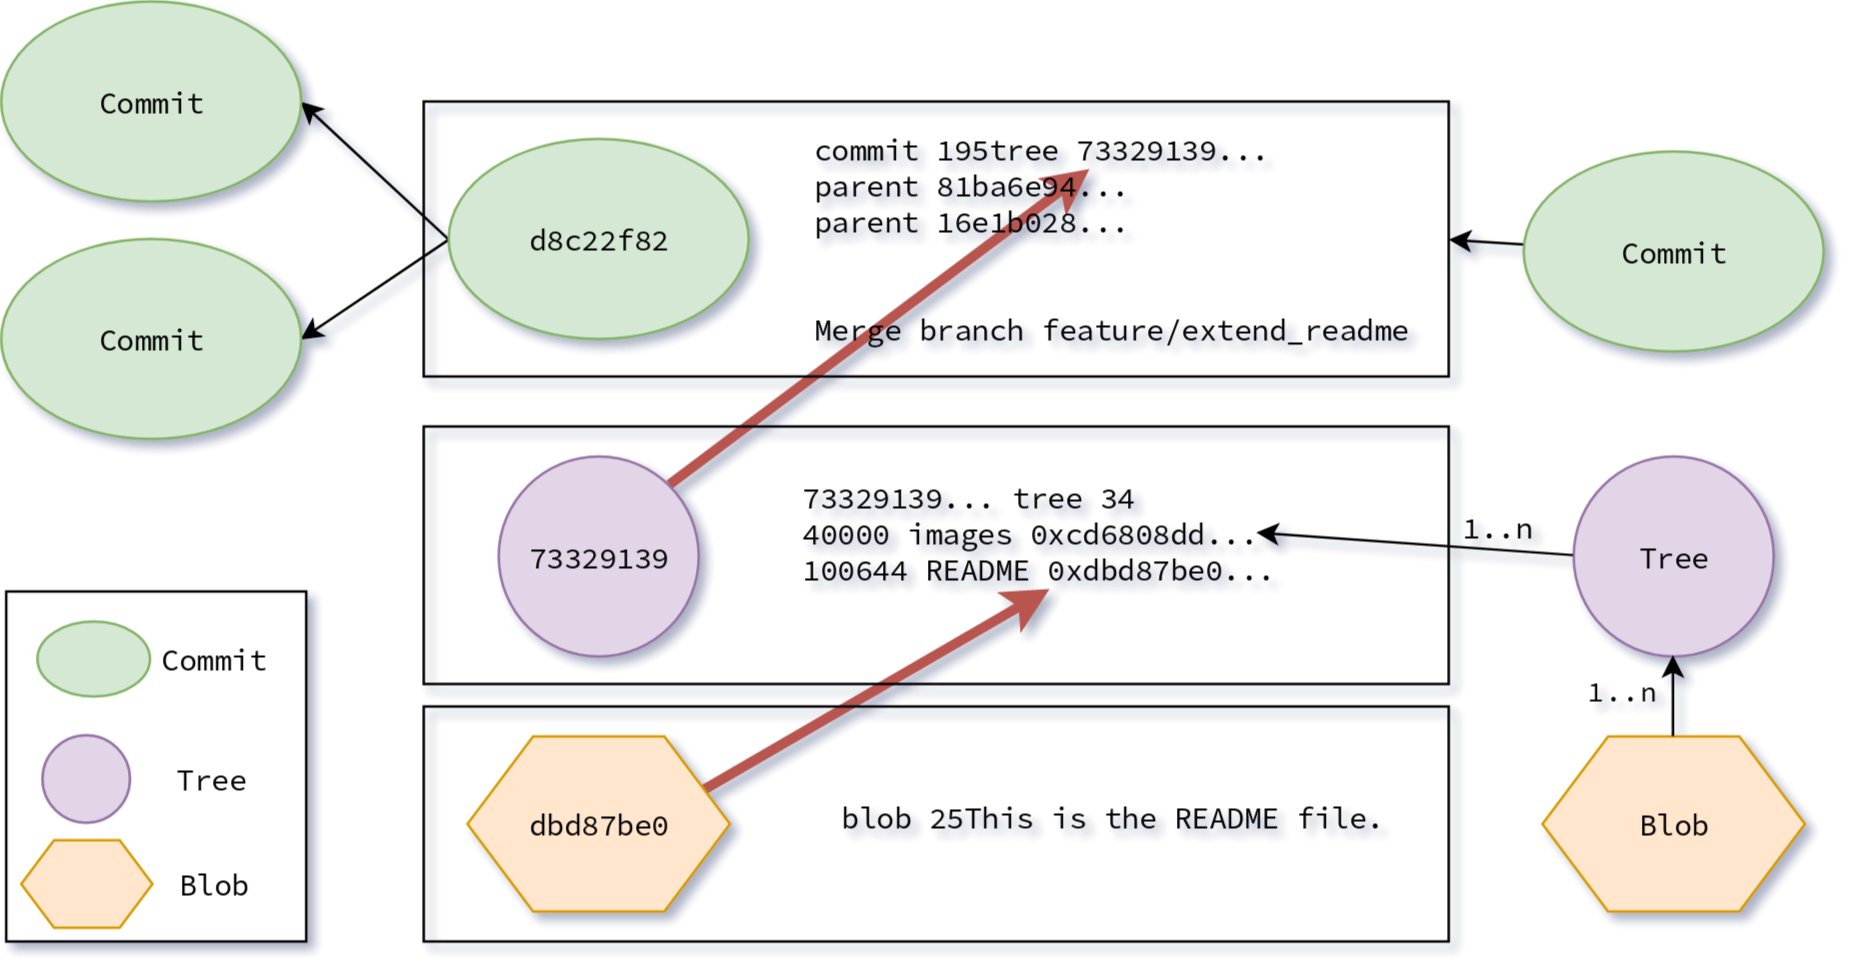
\includegraphics[height=0.70\textheight,keepaspectratio]{./images/Treeish_Blob.png}
            }
            {
                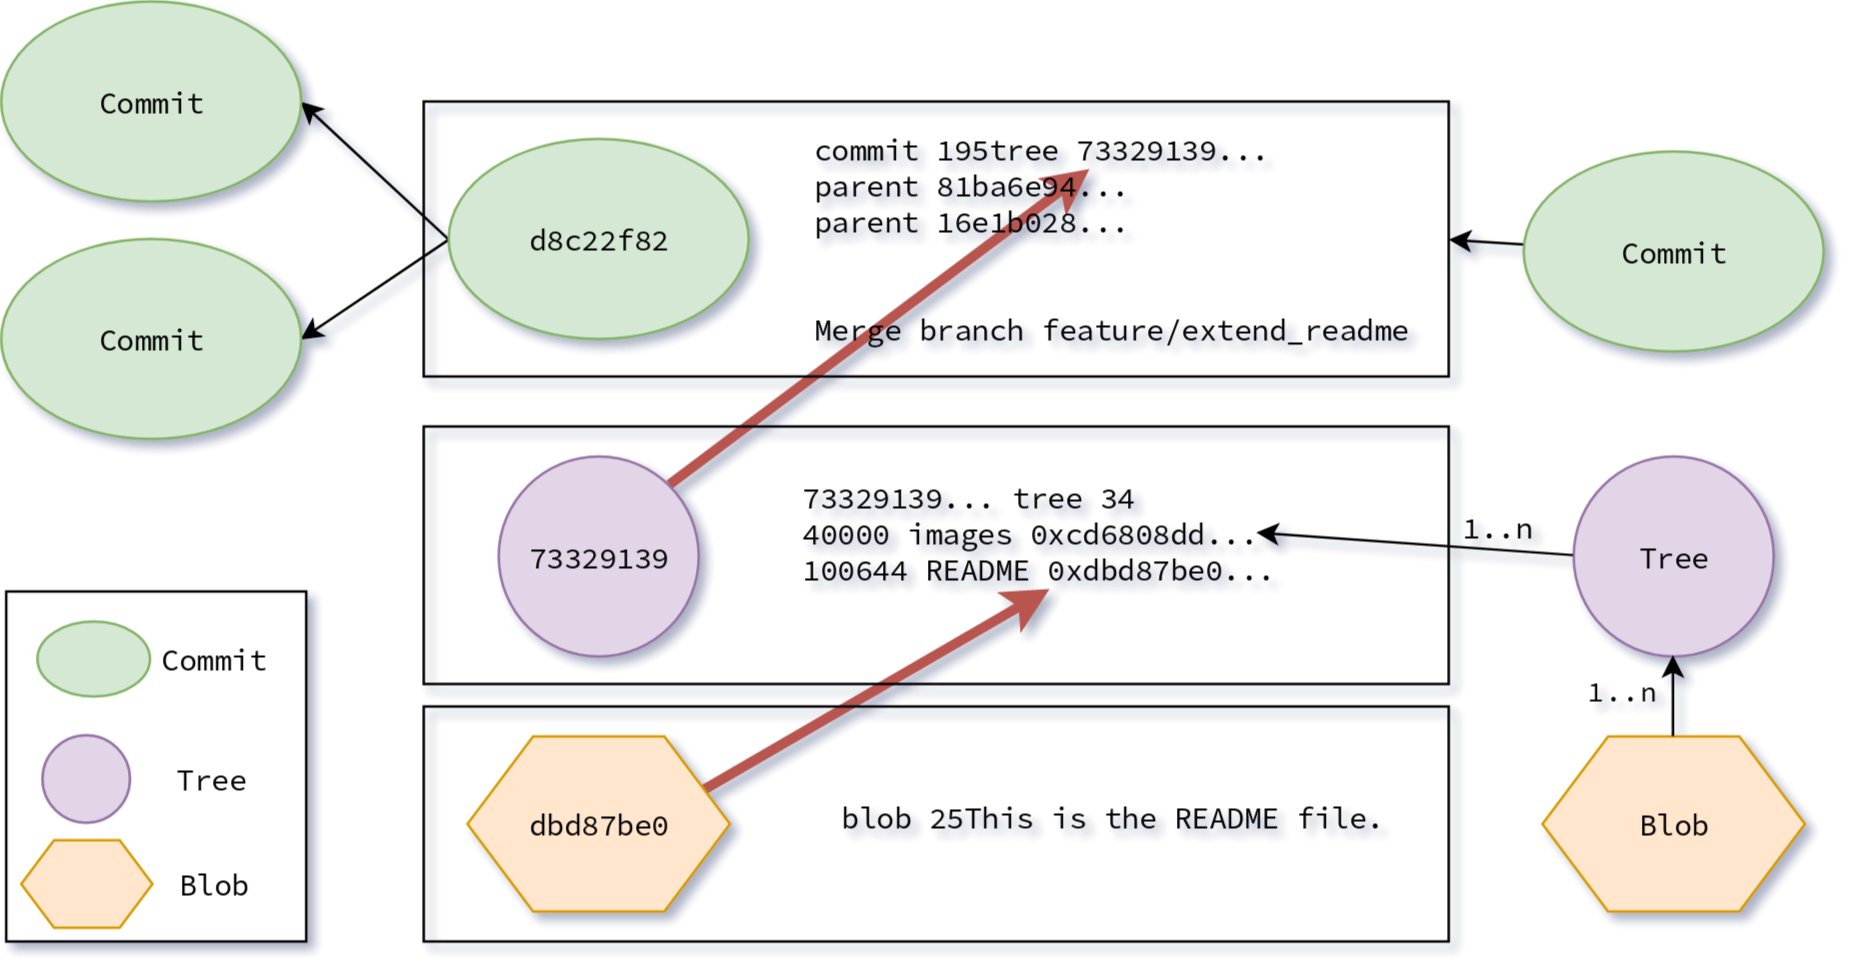
\includegraphics[height=0.6\textheight,width=0.8\textwidth]{./images/Treeish_Blob.png}
            }
            \caption{Git blob}
        \end{center}
    \end{figure}
\end{frame}

